\section{The \lang language}

We now present a formalization of the \lang language featuring
a minimal ML language with let-polymorphism, abstract types, pairs, and our novel
linear type system with borrows which uses kinds and qualified types.
For ease of presentation,
our formalization makes the following simplifications.
First, we only consider matching on pairs, instead of arbitrary algebraic
datatypes. We consider separate operators for borrowing and reborrowing (taking
the borrow of a borrow). We consider regions to be fully annotated
and present a set of rules to infer their placement.
Finally we emulates region variables
as a series of nesting indices.

In the rest of this section, we present the syntax (\cref{syntax}),
a linearity-aware semantics (\cref{sem}), syntax directed typing rules
(\cref{sdtyping}) and automatic rules for region annotations (\cref{regionannot}).

\subsection{Syntax}
\label{syntax}

Let us first define our conventions and meta-syntactic variables.
Expressions, types and kinds are noted respectively $e$, $\tau$, and $k$.
Variables, type variables and kind variables are noted
respectively $x$, $\tvar$ and $\kvar$. Types and kind schemes
are noted $\schm$ and $\kschm$.
In the rest of the text, we will write lists with a bar and an index, for
instance $\Multi[i]{\tau}$.
Kind constants are noted in bold capital letters, such as $\kaff$ for affine.

The syntax of \lang is presented in \cref{grammar} and follows
traditional ML languages with let bindings.
Borrows, noted $\borrow{e}$, are annotated with a specification indicating
if a borrow is immutable ($\IBORROW$) or mutable ($\MBORROW$).
We also distinguish reborrows, which are noted $\reborrow{e}$.
Match are indexed with a specification which can be either $\&^b$
(which $b$ a borrow specification) or $id$, indicating if the match
should operate on borrows or not.
Regions, noted $\region{x}{e}$ are annotated with their nesting ($n$)
and the variable whose borrow they enclose ($x$).
%
$\tapp{t}{\Multi{\tau}}$ denotes a type application where
$\T t$ is an abstract type constructor.
Arrow and borrow types are annotated with a kind, noted $\tau \tarr{k} \tau$
and $\borrowty{k}{\tau}$ respectively.
%
Kinds can be either a kind variable $\kvar$, or constants
(linear $\klin$, affine $\kaff$ or unrestricted $\kun$) indexed
by a nesting level represented by a member of $N \cup \{\infty\}$.
Type schemes and kind schemes are guarded by a set of constraints.
%
Finally, constraints are composed of a list of kind inequalities.


\TODO{Do we explain environments here, or push that for typing, later on ?}

Environments are composed of value and type bindings, along with type
declarations. Type declarations, of the form
$\tydecl{t}{\kschm}{K}{\tau}$, introduce both a new type constructor $\T{t}$ and
a data constructor $K$.

\begin{figure*}[t]
  \centering
  % \begin{subfigure}[t]{0.45\linewidth}
\begin{align*}
  \htag{Expressions}
  e ::=&\ c \mid x \mid \app{e}{e'} \mid \lam{x}{e} \mid \letin{x}{e}{e'}\\
  % |&\ \fix{e}\tag{Fixpoint}\\
  |&\ \introPair{e}{e'} \mid \matchin{x,y}{e}{e'}\tag{Pairs}\\
  |&\ \region{\Sone x\BORROW}{e} \mid \borrow{x} \mid \reborrow{x} \tag{Region \& Borrows}\\
  |&\ \create \mid \observe \mid \update \mid \destroy \tag{Resources}\\
  % |&\ \introK{K}{e}\tag{Data Constructor introduction}\\
  % |&\ \elimK{K}{e}\tag{Data Constructor elimination}\\
  % \htag{Borrows}
  \BORROW ::=& \ \IBORROW % \tag{Shared borrow} \\
  \mid \MBORROW % \tag{Exclusive borrow}\\
  \tag{Borrow specification}\\
  %\htag{Match Specification}
  \etransfm ::=&\ \text{id} % \tag{Normal match} \\
  \mid \&^{\BORROW} % \tag{Borrow match}\\
  \tag{Match Specification}
% \end{align*}
% \end{subfigure}\hfill
% \begin{subfigure}[t]{0.5\linewidth}
% \begin{align*}
  \htag{Types}
  \tau ::=&\ \tvar% \tag{Type variables}\\
  \mid \tyPair{\tau}{\tau'}% \tag{Pair types}\\
  \mid \tapp{\tcon}{\Multi\tau}% \tag{Type constructors}\\
  \tag{ML types}\\
  |&\ \tau\tarr{k}\tau'\tag{Function types}\\
  |&\ \borrowty{k}{\tau}\tag{Borrowed Type}\\
  \htag{Kinds}
  k ::=&\ \kvar \mid \mul_n \hspace{12mm} \forall n \in \Nat \cup \{\infty\} \tag{Kinds}\\
  \mul ::=&\ \klin \mid \kaff \mid \kun\tag{Quality}\\
  \htag{Constrained type and kind schemes}
  C ::=&\ \Multi{\Cleq{k}{k'}}
  \tag{Constraints}\\
  \schm ::=&\ \forall\Multi\kvar\forall\Multi{\bvar{\alpha}{k}}.(\qual{C}{\tau}) \tag{Type scheme}\\
  \kschm ::=&\ \forall\Multi\kvar.(\qual{C}{\Multi{k} \karr k}) \tag{Kind scheme}
\end{align*}
% \end{subfigure}

%%% Local Variables:
%%% mode: latex
%%% TeX-master: "main"
%%% End:

  \caption{Syntax}
  \label{grammar}
\end{figure*}
\begin{figure*}[ht]
\begin{align*}
  \htag{Internal expressions}
  e ::=&\dots \\
  |&\ \lam[k]xe \tag{Kind annotated abstraction} \\
  |&\ \APP e \tau \mid \LAM\tvar v \tag{Type
         application and abstraction}\\
  |&\ \APP ek \mid \LAM\kvar v \tag{Kind application and abstraction}
\end{align*}
\caption{Syntax of internal language}
\label{fig:syntax-internal-language}
\end{figure*}

%%% Local Variables:
%%% mode: latex
%%% TeX-master: "main"
%%% End:


\clearpage
\subsection{Semantics}
\label{sem}

\begin{figure*}[ht]
  % \begin{mathpar}
  \inferrule[Lam]
  { j \fresh }
  { \ered{\closure{j}{x}{e}}{\emptyset}{\lam{x}{e}}{\closure{j}{x}{e}} }
  \and
  \inferrule[App]
  { \ered{I}{E}{f}{\closure{j}{x}{e_f}} \\
    \ered{I'}{E'}{e}{v} \\
    \ered{I''}{E''}{\subst{x}{v}{e_f}}{v_f}
  }
  { \ered{I,I',I''}{E,E',E'',\closure{j}{x}{e_f}}{\app{f}{e}}{v_f} }
  \and
  \inferrule[Let]
  { \ered{I}{E}{e}{v} \\
    \ered{I'}{E'}{\subst{x}{v}{e'}}{v'}
  }
  { \ered{I,I'}{E,E'}{\letin{x}{e}{e'}}{v'} }
\end{mathpar}
%%% Local Variables:
%%% mode: latex
%%% TeX-master: "main"
%%% End:

  \begin{minipage}[t]{0.48\linewidth}
  \begin{align*}
    \htag{Addresses}
    \alpha &::= \ell \tag{Locations}\\
           &\mid \borrow{\alpha} \tag{Borrowed Locations}
    \\
    \htag{Results}
    r &::= \alpha \mid c
  \end{align*}
  \end{minipage}
  \hfill
  \begin{minipage}[t]{0.48\linewidth}
\begin{align*}
    \htag{Storables}
    W &::= (\rho, \closure{k}{x}{e}) \tag{Closures} \\
           &\mid (r, r) \tag{Pairs} \\
    & \mid [r] \tag{Resources}
  \end{align*}
  \end{minipage}
    \begin{mathpar}
    \inferrule{}{ \Sigma, \rho \vdash c \Downarrow \Sigma, c}

    \inferrule{}{\Sigma, \rho \vdash x \Downarrow \Sigma, \rho(x)}

    \inferrule{
      \ell\notin\Dom\Sigma \\
      \Sigma' = \Sigma[\ell \mapsto (\rho, \closure{}{x}{e})]
    }{
      \Sigma, \rho \vdash \lam xe \Downarrow \Sigma', \ell
    }
    
    \inferrule{
      \Sigma, \rho \vdash e \Downarrow \Sigma', \ell \\
      \Sigma' (\ell) = (\rho'',\closure{}{x}{e''}) \\
      \Sigma', \rho \vdash e' \Downarrow \Sigma'', r' \\
      \Sigma'', \rho''[x\mapsto r'] \vdash e'' \Downarrow \Sigma''', r
    }{\Sigma, \rho \vdash \app{e}{e'} \Downarrow \Sigma''', r}

    \inferrule{
      \Sigma, \rho \vdash e \Downarrow \Sigma', r \\
      \Sigma', \rho[x \mapsto r] \vdash e' \Downarrow \Sigma'', r'
    }{
      \Sigma, \rho \vdash \letin{x}{e}{e'} \Downarrow \Sigma'', r'
    }

    \inferrule{
      \Sigma, \rho \vdash e \Downarrow \Sigma', r \\
      \Sigma', \rho \vdash e' \Downarrow \Sigma'', r' \\
      \ell\notin\Dom{\Sigma''} \\
      \Sigma''' = \Sigma''[\ell \mapsto (r, r')]
    }{
      \Sigma, \rho \vdash \introPair{e}{e'} \Downarrow \Sigma''', \ell
    }

    \inferrule{
      \Sigma, \rho \vdash e \Downarrow \Sigma', \ell \\
      \Sigma' (\ell) = (r, r') \\
      \Sigma', \rho[x,y \mapsto r, r'] \vdash e' \Downarrow \Sigma'', r''
    }{
      \Sigma, \rho \vdash \matchin{x,y}{e}{e'} \Downarrow  \Sigma'', r''
    }

    \inferrule{
      \rho (x) = \alpha \\
      \Sigma (\alpha) = W \\
      (\Sigma\setminus\alpha)[\borrow{\alpha} \mapsto W], \rho \vdash e
      \Downarrow \Sigma', r \\
      \Sigma'' = (\Sigma' \setminus\borrow{\alpha})[\alpha \mapsto W]
    }{
      \Sigma, \rho \vdash \region{x}{e} \Downarrow \Sigma', r
    }

    \inferrule{\rho (x) = \alpha}{
      \Sigma, \rho \vdash \borrow{x} \Downarrow \Sigma, \borrow\alpha
    }
    \\
    \inferrule{
      \Sigma, \rho \vdash e \Downarrow \Sigma', r\\
      \ell\notin \Dom\Sigma' }{
      \Sigma,\rho \vdash \create e \Downarrow \Sigma'[\ell \mapsto \rss{r}], \ell
    }

    \inferrule{
      \Sigma, \rho \vdash e \Downarrow \Sigma', \ell \\
      \Sigma' (\ell) = \rss{r}
    }{
      \Sigma, \rho \vdash \destroy e \Downarrow \Sigma'\setminus\ell, ()
    }

    \inferrule{
      \Sigma, \rho \vdash e \Downarrow \Sigma', \borrow[i]\alpha \\
      \Sigma' (\borrow[i]\alpha) = \rss{r}
    }{
      \Sigma, \rho \vdash \observe e \Downarrow \Sigma', r
    }

    \inferrule{
      \Sigma, \rho \vdash e \Downarrow \Sigma', \borrow[m]\alpha \\
      \Sigma', \rho \vdash e' \Downarrow \Sigma'', r' \\
      \Sigma'' (\borrow[m]\alpha) = \rss{r} \\
      \Sigma''' = \Sigma''[\borrow[m]\alpha \mapsto r']
    }{
      \Sigma, \rho \vdash \update e {e'} \Downarrow \Sigma''', ()
    }

  \end{mathpar}
  \caption{Reduction rules -- $\Sigma, \rho, \vdash e \Downarrow
    \Sigma', r$ }
  \label{fig:reduction}
\end{figure*}


%%% Local Variables:
%%% mode: latex
%%% TeX-master: "main"
%%% End:

\begin{figure}
  \lstsemrule{varinst}
  \medskip
  \lstsemrule{sapp}
  \medskip
  \lstsemrule{spair}
  \medskip
  \lstsemrule{sregion}
  \caption{Big-step Interpretation}
\end{figure}


%%% Local Variables:
%%% mode: latex
%%% TeX-master: "main"
%%% End:


\clearpage
\subsection{Typing}
\label{sdtyping}

\subsubsection{Constraint language}

\newcommand\A{\mathcal A}
\newcommand\SC{\mathcal S}

Let us note $\A$ our constraint system. The grammar of constraints is
given in  \cref{grammar:constraint}.
$\A$ is defined as the smallest cylindric term constraint system that
satisfies the axiom shown in \cref{rules:entail}.
We follows the traditional HM(X) formulation
with conjunctions, projections and type inequalities.
The new element specific to our approach are kind inequalities.
Entailment is noted $\entail{C}{D}$, where $D$ is a consequence of the
constraints $C$.
We say that $C$ and $D$ are equivalent, noted $C \equivC D$,
when $\entail{C}{D}$ and $\entail{D}{C}$.
\TODO{Give the cylindric properties ?}

\begin{figure}[tp]
  \centering
  \begin{align*}
    C &::= \Cleq{\tau_1}{\tau_2}
        \mid \Cleq{k_1}{k_2}
        \mid C_1 \Cand C_2
        \mid \Cproj{\tvar}{C}
        \mid \Cproj{\kvar}{C}
  \end{align*}
  \caption{The constraint language}
  \label{grammar:constraint}
\end{figure}

\begin{figure*}[tp]
  \begin{minipage}{0.65\linewidth}
  \begin{mathpar}
    \inferrule[Lat-UA]{}{\kun_n \lk_\Lat \kaff_n}
    \and
    \inferrule[Lat-AL]{}{\kaff_n \lk_\Lat \klin_n}
    \and
    \inferrule[Lat-U-Level]{n \lk n'}{\kun_n \lk_\Lat \kun_{n'}}
    \and 
    \inferrule[Lat-A-Level]{n \lk n'}{\kaff_n \lk_\Lat \kaff_{n'}}
    \and 
    \inferrule[Lat-L-Level]{n \lk n'}{\klin_n \lk_\Lat \klin_{n'}}
  \end{mathpar}
\end{minipage}~
\begin{minipage}{0.2\linewidth}
  \centering
  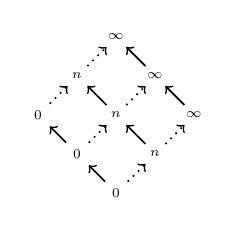
\begin{tikzpicture}
    [->,auto,semithick, every node/.style={scale=0.7}]
    \node(U) {$\kun_0$} ;
    \node(A) [above left of=U] {$\kaff_0$} ;
    \node(L) [above left of=A] {$\klin_0$} ;
    \node(Un) [above right of=U] {$\kun_n$} ;
    \node(An) [above left of=Un] {$\kaff_n$} ;
    \node(Ln) [above left of=An] {$\klin_n$} ;
    \node(Uinf) [above right of=Un] {$\kun_\infty$} ;
    \node(Ainf) [above left of=Uinf] {$\kaff_\infty$} ;
    \node(Linf) [above left of=Ainf] {$\klin_\infty$} ;
    \path
    (U) edge (A)
    (A) edge (L)
    (Un) edge (An)
    (An) edge (Ln)
    (Uinf) edge (Ainf)
    (Ainf) edge (Linf)
    ;
    \path[dotted]
    (U) edge (Un)
    (A) edge (An)
    (L) edge (Ln)
    (Un) edge (Uinf)
    (An) edge (Ainf)
    (Ln) edge (Linf)
    ;
  \end{tikzpicture}
\end{minipage}

%%% Local Variables:
%%% mode: latex
%%% TeX-master: "../main"
%%% End:

  \caption{Lattice inequalities -- $k \lk_\Lat k'$}
  \begin{mathpar}
  \inferrule{l \leq_{\mathcal L} l'}{\entail{}{\Cleq{l}{l'}}}
  \and
  \inferrule{}{\entail{}{\Cleq{k}{\klin_\infty}}}
  \and
  \inferrule{}{\entail{}{\Cleq{\kun_0}{k}}}
  \and
  \inferrule
  {}{ \entail{}{\Cleq{\kvar}{\kvar}} }
  % \and
  % \inferrule
  % {\Cleq{k}{k'} \in C}{ \entail{C}{\Cleq{k}{k'}} }
  % \and
  % \inferrule
  % { \entail{C}{\Cleq{x_1}{x}}\\
  %   \entail{C}{\Cleq{x}{x_2}}
  % }
  % { \entail{C}{\Cleq{x_1}{x_2}} }
  % \and
  % \inferrule
  % { \entail{C}{D} }
  % { \entail{C}{\Cproj{x}{D}} }
  \\
  \inferrule
  { \entail{C}{\Cleq{\tau'_1}{\tau_1}}\\
    \entail{C}{\Cleq{\tau_2}{\tau'_2}}\\
    \entail{C}{\Cleq{k}{k'}}
  }
  { \entail{C}{\Cleq{\tau_1\tarr{k}\tau_2}{\tau'_1\tarr{k'}\tau'_2}} }
  \and
  \inferrule
  { \forall i,\ \entail{C}{\Ceq{\tau_i}{\tau_i}}\\
  }
  { \entail{C}{\Cleq{\tapp{t}{(\tau_i)}}{\tapp{t}{(\tau'_i)}}} }
  % \and
  % \inferrule
  % { \entail{C}{\Cleq{k}{k'}} \\
  %   \entail{C}{\Cleq{k'}{k}} }
  % { \entail{C}{\Ceq{k}{k'}} }
  % \and
  % \inferrule
  % { \entail{C}{\Cleq{k}{k'}} }
  % { \entail{C}{\Ckind{\tau_0\tarr{k}\tau_1}}{k'}}
  % \and
  % \text{Completion to form a cylindric constraint system.}
\end{mathpar}

%%% Local Variables:
%%% mode: latex
%%% TeX-master: "../main"
%%% End:

  \caption{Base entailment rules -- $\entail{C}{D}$ }
  \label{rules:entail}
\end{figure*}


We note $\SC$ the set of solved forms
which can be used inside type and kind schemes.
We define $\SC$ as $\A$ quotiented by the relation $\equivC$.
%
We consider the existence of a function $\operatorname{normalize}$ which takes
a constraint in $\A$ and a substitution $\psi$ and returns a constraint
in solved form $C' \in \SC$,
and an updated substitution. We detail the implementation
of the normalization function in \cref{sec:normalize}

% $\mathcal S$ is composed only of kind
% inequalities \emph{over variables}. For convenience, if $C\in\mathcal S$, we
% note $C$ as a list of kind inequalities: $\Cleq{\kvar_i}{\kvar_{i'}}^n$.
% \TODO{Extend the properties of solved forms}

\subsubsection{Kinding}

We note $\inferSK{C}{\E}{\tau}{k}$
when $\tau$ has kind $k$ in environment $\E$ under constraints $C$.
The rules are shown in \cref{rules:sd-kinding}.
Kinds and types follow a small calculus with variables ($\tvar$,\dots),
functions (type constructors $\T{t}$), application ($\tapp{t}{\Multi{\tau}}$)
and primitives such as arrow ($\tau\tarr{k}\tau'$) and
borrow ($\borrowty{k}{\tau}$).
Kind inference is thus fairly straightforward and is done simply by following
the syntax of the types. The only kind arrows can appear when looking
up the kind scheme of a type constructor $\T t$. Kind arrows are forbidden
in any other contexts.


\begin{figure}[ht]
  \centering
  \begin{mathpar}
  \inferrule[KVar]
  { \bvar{\tvar}{k} \in \E }
  { \inferSK{C}{\E}{\tvar}{k}
  }
  \and
  \inferrule[KArr]
  {}
  { \inferSK{C}{\E}{\tau_1 \tarr{k} \tau_2}{k} }
  \and
  \inferrule[KApp]
  { \bvar{\T{\tcon}}{
      \forall \Multi[i]\kvar.\ \qual{D}{(\Multi[j]{k'}) \karr k'}}
    \in \E \\
    \inferSK{C}{\E}{\Multi[j]{\tau}}{\Multi[j]{k}} \\
    \unif = \subst{\Multi[i]\kvar}{\Multi[i]k}{} \\
    \entail C {\unif D} \\
    \inferSS{C}{\E}{\Multi[j]k}{\unif{\Multi[j]{k'}}}
  }
  { \inferSK{C}{\E}{\tapp{\tcon}{\Multi[j]{\tau}}}{\unif{k'}} }
  \and
  \inferrule[KBorrow]
  {}{ \inferSK{C}{\E}{\borrowty{k}{\tau}}{k}}
  \and
  \inferrule[KPair]
  { \forall i \quad
    \inferSK{C}{\E}{\tau_i}{k_i} \quad
    \inferSS{C}{\E}{k_i}{k}
  }
  { \inferSK{C}{\E}{\tyPair{\tau_1}{\tau_2}}{k} }
\end{mathpar}


%%% Local Variables:
%%% mode: latex
%%% TeX-master: "../main"
%%% End:

  \caption{Syntax-directed kinding rule --
    $\inferSK{C}{\E}{\tau}{k}$}
  \label{rules:sd-kinding}
\end{figure}

\subsubsection{Environments}


\begin{figure}[tp]
  \begin{minipage}{0.38\linewidth}
\begin{mathpar}
  \inferrule[ESplit-Empty]{}{
    \bsplit{\Cempty}\Eempty\Eempty\Eempty
  }

  \inferrule[ESplit-Nonempty]{
    \bsplit{C_1}{\E}{\E_1}{\E_2} \\
    \bsplit{C_2}{b}{b_1}{b_2}
  }{
    \bsplit{C_1\Cand C_2}{\E;b}{\E_1;b_1}{\E_2;b_2}
  }

  \inferrule[ESplit-Check]{
    \bsplit{D}{\E}{\E_1}{\E_2} \\
    \entail{C}{D}
  }{
    \lsplit{C}{\E}{\E_1}{\E_2}
  }
\end{mathpar}
\end{minipage}\vrule~
\begin{minipage}{0.6\linewidth}
    \begin{tabular}
      {@{}>{$}r<{$}@{ $\Lleftarrow$ }
      >{$}c<{$}@{ $=$ }
      >{$}c<{$}@{ $\ltimes$ }
      >{$}c<{$}r}
      
      \Cleq{\schm}{\kun_\infty}
      &\bvar{x}{\schm}&\bvar{x}{\schm}&\bvar{x}{\schm}
      &Both\\[2mm]

      {\Cempty}&
      {\bvar{\borrow[\IBORROW]{x}}{\schm}}&
      {\bvar{\borrow[\IBORROW]{x}}{\schm}}&{\bvar{\borrow[\IBORROW]{x}}{\schm}}
      &Borrow\\[2mm]

      {\Cempty}&{\bvar{x}{\schm}}&{\bvar{x}{\schm}}&{\bnone}
      &Left\\
      {\Cempty}&{\bvar{x}{\schm}}&{\bnone}&{\bvar{x}{\schm}}
      &Right\\[2mm]

      {\Cempty}&{\bvar x \schm}&{\svar x \schm^n}&{\bvar x \schm}
      &Susp\\

      {\Cempty}&
      {\bvar{\borrow x} \schm}&{\svar[\IBORROW] x \schm^n}&{\bvar{\borrow x} \schm}
      &SuspB\\

    \end{tabular}
\end{minipage}

% \begin{mathpar}
%   \inferrule[BSplit-Both]{}{
%     \bsplit {\Cleq{\schm}{\kun_\infty}}
%     {\bvar{x}{\schm}} {\bvar{x}{\schm}} {\bvar{x}{\schm}}
%   }

%   \inferrule[BSplit-Left]{}{
%     \bsplit {\Cempty} {\bvar{x}{\schm}} {\bvar{x}{\schm}} {\bnone}
%   }

%   \inferrule[BSplit-Right]{}{
%     \bsplit {\Cempty} {\bvar{x}{\schm}} {\bnone} {\bvar{x}{\schm}}
%   }

%   \inferrule[BSplit-Imm-Borrow]{}{
%     \bsplit {\Cempty}
%     {\bvar{\borrow[\IBORROW]{x}}{\schm}}
%     {\bvar{\borrow[\IBORROW]{x}}{\schm}}{\bvar{\borrow[\IBORROW]{x}}{\schm}}
%   }

%   \inferrule[BSplit-To-Borrow]{}{
%     \bsplit {\Cempty}{\bvar x \schm}{\svar x \schm^n}{\bvar x \schm}
%   }

%   \inferrule[BSplit-To-Imm]{}{
%     \bsplit {\Cempty}
%     {\bvar{\borrow x} \schm}{\svar[\IBORROW] x \schm^n}{\bvar{\borrow x} \schm}
%   }
% \end{mathpar}
%%% Local Variables:
%%% mode: latex
%%% TeX-master: "../main"
%%% End:

  \caption{Splitting --- environments $\lsplit
    C\E\E\E$; binders $\bsplit Cbbb$}
  \label{fig:sd-splitting}
\end{figure}

\begin{figure}[tp]
  \begin{mathpar}
  \inferrule[EBorrow]{
    \bregion{C_r}{}{\svar{x}{\tau}^n}{b}
  }{
    \bregion{C_r}{x}{\E;\svar{x}{\tau}^n}{\E; b}
  }

  \inferrule[EBorrow-Check]{
    \bregion{D}{x}{\E;\svar{x}{\tau}^n}{\E; b} \\
    \entail{C}{D}
  }{
    \lregion{C}{x}{\E;\svar{x}{\tau}^n}{\E; b}
  }
\end{mathpar}
\hrulefill
\begin{mathpar}
  \inferrule[BSplit-Immut]{}{
    \bregion{(\kun_n\lk k\lk\kun_\infty)}{}
    {\svar[\IBORROW]{x}{\tau}^n}{\bvar{\borrow[\IBORROW]{x}}{\borrowty[\IBORROW] k{\tau}}}
  }
  \and
  \inferrule[BSplit-Mut]{}{
    \bregion{(\kaff_n\lk k\lk\kaff_\infty)}{}
    {\svar[\MBORROW]{x}{\tau}^n}{\bvar{\borrow[\MBORROW]{x}}{\borrowty[\MBORROW] k{\tau}}}
  }
\end{mathpar}
%%% Local Variables:
%%% mode: latex
%%% TeX-master: "../main"
%%% End:

  \caption{Borrowing --- environments $\lsplit
    C\E\E\E$; binders $\bsplit Cbbb$}
  \label{fig:sd-borrowing}
\end{figure}

\subsubsection{Typing}

\begin{figure*}[tp]
  \begin{mathpar}
  \inferrule{}{ \Cleq{\Eempty}{k} = \Cempty}

  \inferrule{
    \Cleq\E k = C_1 \\ \Cleq B k = C_2
  }{
    \Cleq{\E; B}{k} = C_1 \Cand C_2
  }

  \inferrule{
    \Cleq \tau k = C
  }{ \Cleq{\bvar x \tau}{k} = C}

  \inferrule{
    \Cleq \tau k = C_1 \\
    \BORROW ??? C_2
  }{
    \Cleq{\svar x \tau} k = C_1 \Cand C_2
  }

  \inferrule{}
  { \Cleq{ \tau_2\tarr{k'}\tau_1 } k = \Cleq{k'}k }

  \inferrule{
    \tvar : \kschm
  }
  { \Cleq{ \tvar} k = \Cleq\kschm k }

  \inferrule{
  }{ \Cleq{\tapp{t}{\Multi\tau}} k = ???}

  \inferrule{}{
    \Cleq{\borrow{\tau}} k = ???
  }
\end{mathpar}

%%% Local Variables:
%%% mode: latex
%%% TeX-master: "../main"
%%% End:

  \caption{Rewriting constraints on environments and types}
  \label{fig:contraints-environments-types}
\end{figure*}
\begin{figure*}[tp]
  % \begin{mathpar}
%   \inferrule[Scheme]{
%     \inferSK{C \Cand C_x} \E \tau {k'} \\
%     \entail C {\Cleq{k'}k}
%   }{
%     \entail C {(\forall \kvar_i \forall (\tvar_j:k_j).\
%       \qual{C_x}{\tau}) \le  k}
%   }
% \end{mathpar}
% \hrulefill
\begin{mathpar}
  \ruleSDConst
  \and
  \ruleSDVar
  \and
  \ruleSDLam
  \and
  \ruleSDBorrow
  \and
  \ruleSDReBorrow
  \and
  \ruleSDPair
  \and
  \ruleSDRegion
  \and
  \ruleSDApp
  \and
  \ruleSDLet
  \and
  \ruleSDMatchPair
  \and
  \ruleSDCreate
  \and
  \ruleSDObserve
  \and
  \ruleSDUpdate
  \and
  \ruleSDDestroy
  % \and
  %
  %
  % \inferrule[Elim]
  % { \tvar,(\kvar'_i),(\tvar'_j)\text{ new}\\
  %   \bvar{K}{
  %     \forall \kvar_i \forall (\tvar_j:\kvar_j).\ \qual{C_K}{\tau_1 \tarr{}\tau_2}
  %   } \in \E\\
  %   \inferW{\Sv}{(C,\unif)}{\E}{e}{\tau} \\
  %   \unif' =
  %   \subst{\kvar_i}{\kvar'_i}{} \meet
  %   \subst{\tvar_j}{\tvar'_j}{} \meet \unif \\
  %   D =
  %   C \Cand C_K \Cand \Cleq{\tau_1}{\tvar} \Cand \Cleq{\tau}{\tau_2} \\
  %   (C,\unif) = \normalize{D}{\unif'}\\
  % }
  % { \inferW{\addlin{\Sv}}{(C,\unif|_{\fv{\E}})}{\E}{\elimK{K}{e}}
  %   {\unif\tvar} }
\end{mathpar}

% \begin{align*}
%   \Weaken(x,\Sv)
%   &\equiv \begin{cases}
%     \operatorname{kind}(x)\lk\kun &\text{if } \operatorname{kind}(x)\in\Sv\\
%     \Cempty &\text{otherwise}
%   \end{cases}\\
%   \Cleq{\Sv}{k}
%   &\equiv \bigwedge_{\kvar\in\Sv} \Cleq{\kvar}{k}
% \end{align*}

%%% Local Variables:
%%% mode: latex
%%% TeX-master: "../main"
%%% End:

  \caption{Syntax-directed typing rules}
  \label{fig:syntax-directed-typing}
\end{figure*}

\clearpage

\subsection{Annotating regions}
\label{regionannot}

So far, all \lang programs have been fully annotated with regions information.
We now show how to infer these regions annotations based on
optionally-annotated programs.
First, we extend the region annotation to $\region{S}{E}$ where $S$ is
a set of variables. This annotation, defined below, is equivalent to nested
region annotations for each individual variable.

\begin{align*}
  \region{x;S}{e} &= \region{x}{\region{S}{e}}& \region{\emptyset}{e} &= e\\
\end{align*}

\Cref{fig:region-annotation} define a rewriting relation $\RannotT{e}{e'}$
which indicates that an optionally annotated term $e$ can be written
in a fully annotated term $e'$.
Through the rule \textsc{Rewrite-Top}, this is defined
in term of an inductively defined relation
$\Rannot{e}{e'}{S}$ where $n$ is the current nesting and $S$ is a set of
variable that are not enclosed in a region yet.
The base cases are constants, variables and borrows.
The general idea is to start from the leafs of the syntax tree, create a
region for each borrow, and enlarge the region as much as possible.
This is implemented by a depth-first walk of the syntax
tree which collects each variable that has a corresponding borrow.
At each step, it rewrites the inner subterms,
consider which borrow must be enclosed by a region now, and
return the others for later enclosing. Binders force immediate
enclosing of the bound variables, as demonstrated in rule \textsc{Rewrite-Lam}.
For nodes with multiple children, we
use a scope merge operator to decide if regions should be placed and where.
This is shown in rule \textsc{Rewrite-Pair}.
The merge operator, written $\getBorrows{B_l}{B_r}{(S_l,S,S_r)}$, takes
the sets $B_l$ and $B_r$ returned by rewriting the subterms
and returns three sets: $S_l$ and $S_r$ indicates the variables
that should be immediately enclosed by a region on the left and right
subterms and $S$ indicates the set of the yet-to-be-enclosed variables.
As an example, the rule \textsc{AnnotRegion-MutLeft} is applied
when there is an immutable borrow and a mutable borrow. In that case, a
region is created to enclose the immutable borrow, while the mutable
borrow is left to be closed later. This is coherent with the rules
for environment splitting and suspended bindings from \cref{sdtyping}.
%
Explicitly annotated regions are handled specially through
rule \textsc{Rewrite-Region}. In that case, we assume that all inner
borrows should be enclosed immediately.

\begin{figure*}[htp]
  \centering
  \begin{mathpar}
  \inferrule[AnnotRegion-Empty]{}{
    \getBorrows{\Sempty}{\Sempty}{\Sempty,\Sempty,\Sempty}
  }

  \inferrule[AnnotRegion-Nonempty]{
    \getBorrows{B_1}{B_2}{S_1,S,S_2}\\
    \getBorrows{b_1}{b_2}{S'_1,S',S'_2}
  }{
    \getBorrows{B_1;b_1}{B_2;b_2}
    {S_1\Sunion S'_1,S\Sunion S',S_2\Sunion S'_2}
  }
\end{mathpar}
\hrulefill
\begin{mathpar}
  \inferrule[AnnotRegion-Left]{}{
    \getBorrows
    {\Sone{x}{b}}
    {\Cempty}
    {\Cempty,\Sone{x}{b},\Cempty}
  }
  
  \inferrule[AnnotRegion-Right]{}{
    \getBorrows
    {\Cempty}
    {\Sone{x}{b}}
    {\Cempty,\Sone{x}{b},\Cempty}
  }
  
  \inferrule[AnnotRegion-Immut]{}{
    \getBorrows
    {\Sone{x}{\IBORROW}}
    {\Sone{x}{\IBORROW}}
    {\Cempty,\Sone{x}{\IBORROW},\Cempty}
  }
  
  \inferrule[AnnotRegion-MutLeft]{}{
    \getBorrows
    {\Sone{x}{\IBORROW}}
    {\Sone{x}{\IBORROW}}
    {\Sone{x}{\IBORROW},\Sone{x}{\MBORROW},\Cempty}
  }
  
  \inferrule[AnnotRegion-MutRight]{}{
    \getBorrows
    {\Sone{x}{\MBORROW}}
    {\Sone{x}{\IBORROW}}
    {\Cempty,\Sone{x}{\MBORROW},\Sone{x}{\IBORROW}}
  }
  
  \inferrule[AnnotRegion-Mut]{}{
    \getBorrows
    {\Sone{x}{\MBORROW}}
    {\Sone{x}{\MBORROW}}
    {\Sone{x}{\MBORROW},\Cempty,\Sone{x}{\IBORROW}}
  }
\end{mathpar}
\hrulefill
\begin{mathpar}
  \inferrule{}
  { \Rannot{\borrow{x}}{\borrow{x}}{\Sone{x}{b}} }

  \inferrule
  { \forall i,\ \Rannot{e_i}{e'_i}{B_i} \\
    \getBorrows{B_1}{(B_2\Sdel{x})}{S_1,S,S_2} \\
    S'_2 = S_2\Sunion B_2\Sonly{x}
  }
  { \Rannot
    {\letin{x}{e_1}{e_2}}
    {\letin{x}{\region{S_1}{e'_1}}{\region{S'_2}{e'_2}}}{S} }
  
  \inferrule{e = c\ |\ x}
  { \Rannot{e}{e}{\Sempty} }

  \inferrule
  { \forall i,\ \Rannot{e_i}{e'_i}{B_i} \\
    \getBorrows{B_1}{B_2}{S_1,S,S_2}
  }
  { \Rannot{\app{e_1}{e_2}}{\app{\region{S_1}{e'_1}}{\region{S_2}{e'_2}}}{S} }

  \inferrule
  { \Rannot{e}{e'}{B} \\
    B_x = B\Sonly{x}
  }
  { \Rannot{\lam{x}{e}}{\lam{x}{\region{B_x}{e'}}}{B\Sdel{x}} }

  \inferrule
  { \Rannot{e}{e'}{B} }
  { \Rannot{\regionS{e}}{\region{B}{e'}}{\Sempty} }

  \inferrule
  { \forall i,\ \Rannot{e_i}{e'_i}{B_i} \\
    \getBorrows{B_1}{B_2}{S_1,S,S_2}
  }
  { \Rannot
    {\introPair{e_1}{e_2}}
    {\introPair{\region{S_1}{e'_1}}{\region{S_2}{e'_2}}}
    {S} }

  \inferrule
  { \forall i,\ \Rannot{e_i}{e'_i}{B_i} \\
    \getBorrows{B_1}{(B_2\Sdel{x,y})}{S_1,S,S_2} \\
    S'_2 = S_2\Sunion B_2\Sonly{x,y}
  }
  { \Rannot
    {\matchin{x,y}{e_1}{e_2}}
    {\matchin{x,y}{\region{S_1}{e'_1}}{\region{S'_2}{e'_2}}}{S} }
\end{mathpar}

%%% Local Variables:
%%% mode: latex
%%% TeX-master: "main"
%%% End:

  \caption{Automatic region annotation --- $\RannotT{e}{e'}$}
  \label{fig:region-annotation}
\end{figure*}

%%% Local Variables:
%%% mode: latex
%%% TeX-master: "main"
%%% End:
